\htwo{Handbuch Server}
\hthree{Installation}

Der \ZELIA\ Server ist notwendig um den \ZELIA\ Client zu verwenden, da der Client eine Web-Applikation ist und diese vom \ZELIA\ Server bereit gestellt wird. Zusätzlich stellt dieser Server die ZELIA-API zur Verfügung, welche vom Client verwendet wird um Informationen der Räume abzufragen und zu schreiben. Die Datenbank, in der Informationen über die Räume gespeichert sind, wird auch mittels Container direkt auf diesem Server gestartet.

\hfour{Abhänigkeiten}

\hfive{NodeJS}

Bevor man den Server aufsetzen und verwenden kann, gibt es ein paar Abhängigkeiten die man installieren sollte. Die wichtigste Abhängigkeit, die man nur zum Entwickeln braucht, ist NodeJS. NodeJS ist eine Javascript Engine, welche ohne ein Browser-Frontend läuft (siehe Kapitel NodeJS \ref{sec:nodejs}). Installieren kann man NodeJS einfach von der offiziellen Webseite \emph{https://nodejs.org/} (siehe Abbildung \ref{fig:nodejsdownload}). Die Version 16.14.0 bietet sich an, da die meisten Pakete diese Version unterstützen. Für \ZELIA\ macht es aber keinen Unterschied, welche Version verwendet wird, da der Server auch auf der neusten Version von Node läuft.

\begin{figure}[H]
    \centering
    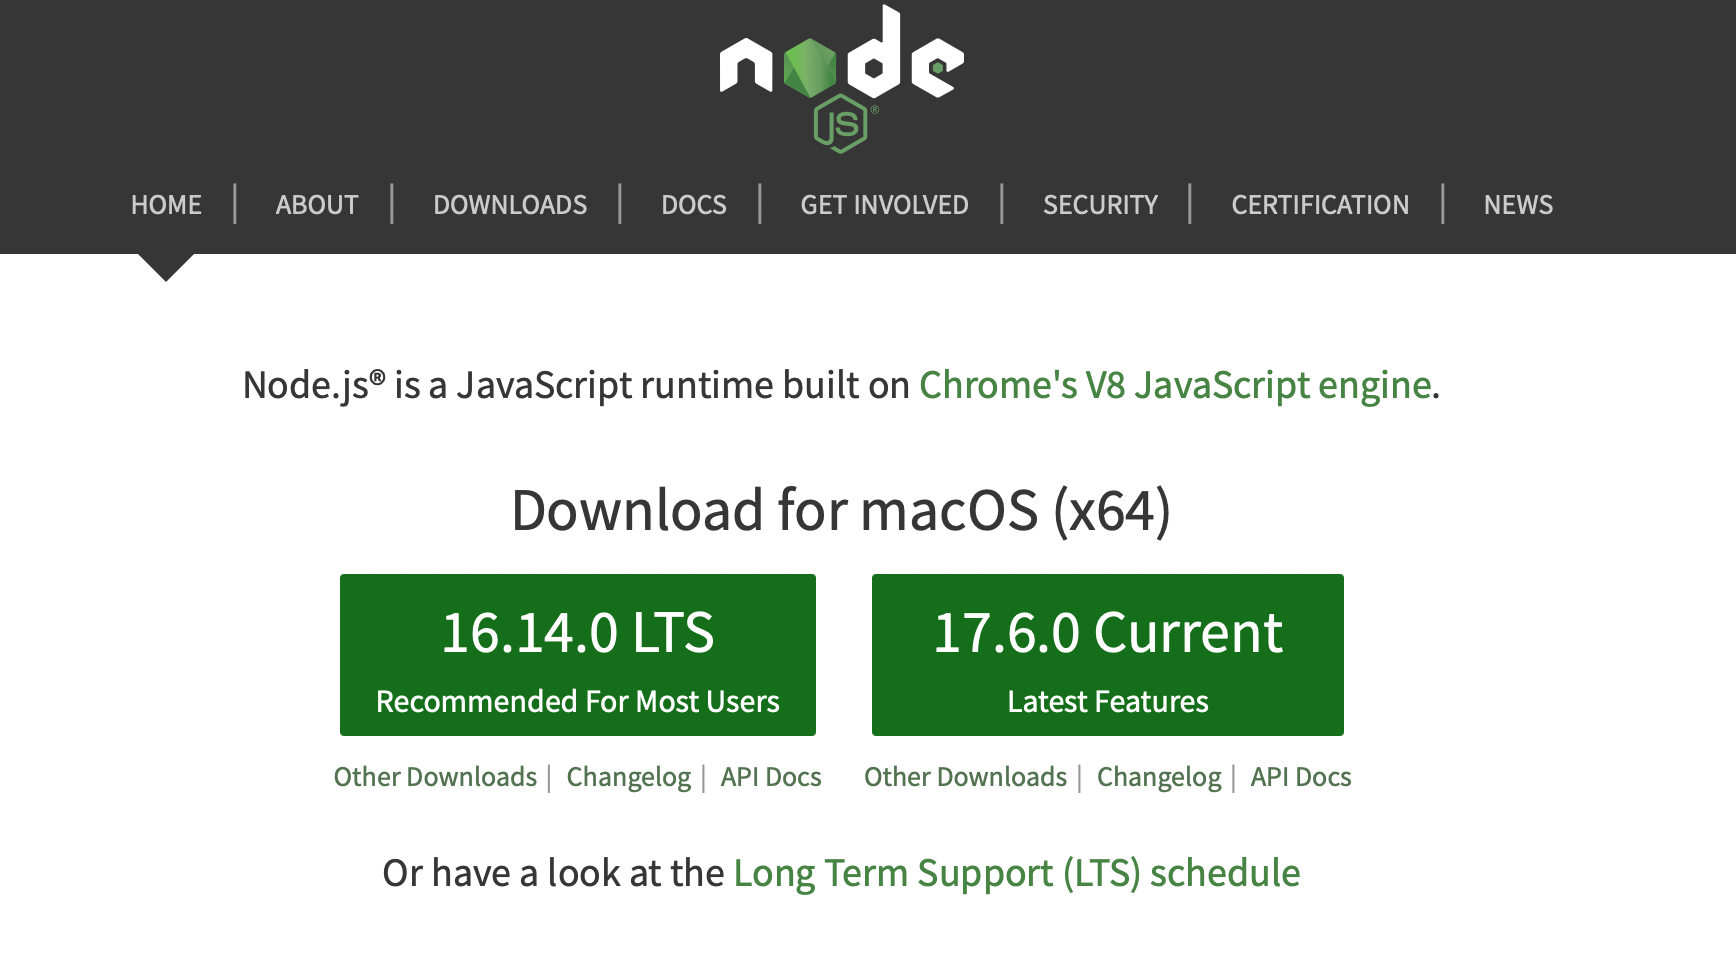
\includegraphics[width=120mm]{media/Handbuch/nodejs.png}
    \caption{Installation von NodeJS}
    \label{fig:nodejsdownload}
\end{figure}

\hfive{Git}

Durch die Installation von Git, kann man sich das Arbeiten mit dem Quellcode erleichtern, notwendig ist es aber nicht. Verwenden kann man das Programm als Befehl in der Konsole. Unter den Meisten Linux Distributionen ist Git bereits vorinstalliert. Unter MacOS kann man Git herunterladen, wenn man die Apple Entwicklungswerkzeuge installiert, welche mit der Entwicklerumgebung Xcode mitgeliefert werden. Um Git auf Windows laufen zu lassen, kann man das Programm von der offiziellen Website \emph{https://git-scm.com/downloads} herunterladen.

GitHub stellt "GitHub Desktop" zur Verfügung, welches auch ein integriertes Git mitbringt. Zusätzlich hat "GitHub Desktop" eine grafische  Benutzeroberfläche, die den Einstieg in GitHub und Git vereinfachen kann (\emph{https://desktop.github.com}). 

\begin{figure}[H]
    \centering
    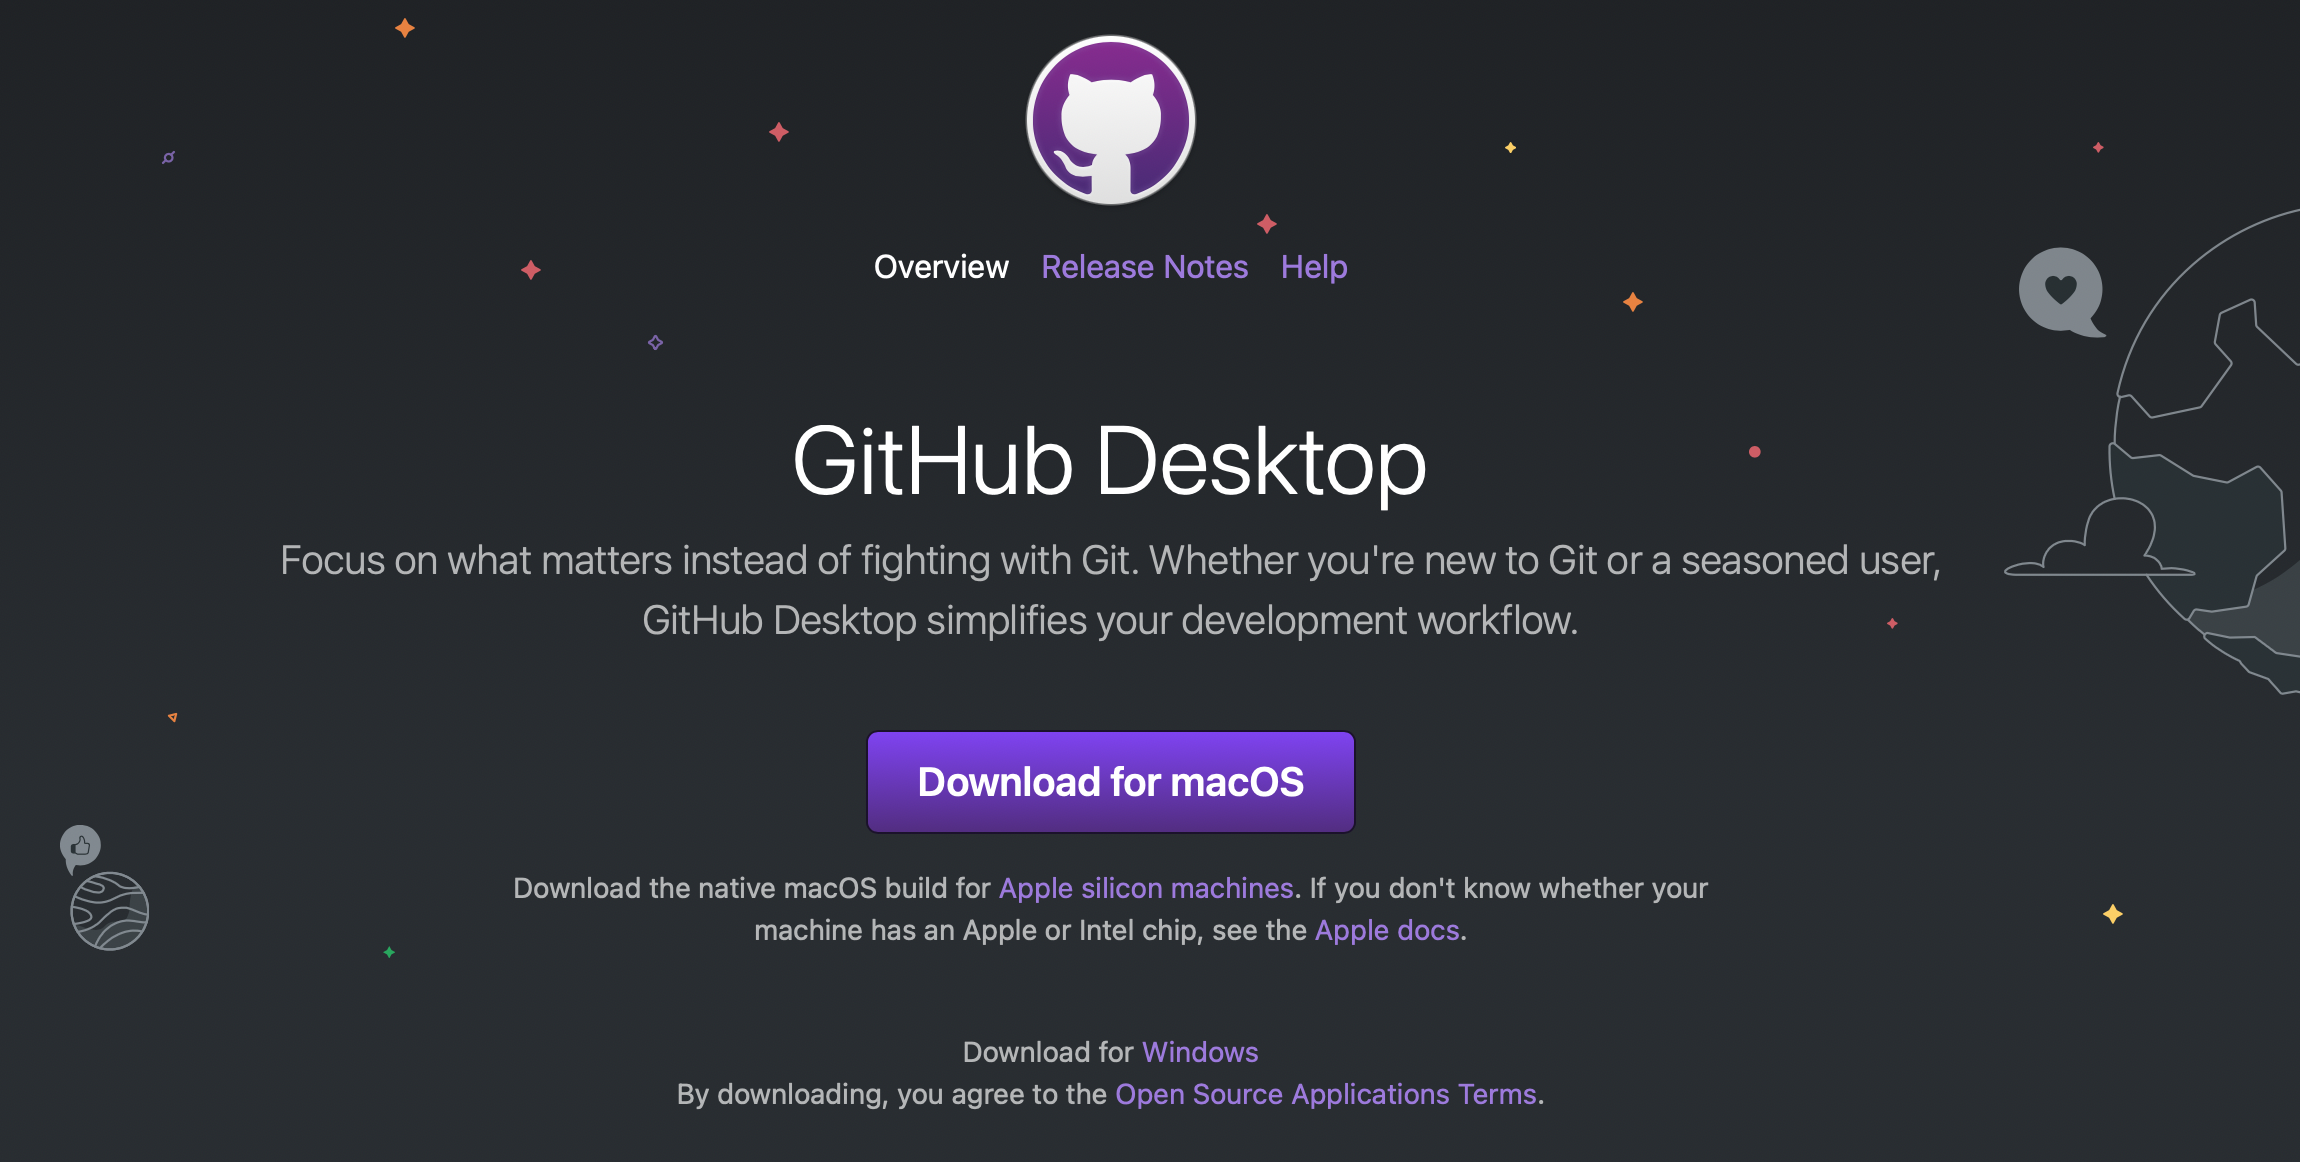
\includegraphics[width=100mm]{media/Handbuch/github_desktop.png}
    \caption{Installation von "GitHub Desktop"}
    \label{fig:githubdesktop}
\end{figure}

\hfive{Docker}

Docker baut, wie man in Kapitel \ref{sec:ContainerAndDocker} erfährt, auf Containertechnologien auf, die es möglich machen unabhängig von der Hardware ausgeführt zu werden. Rein theoretisch bräuchte man Docker nicht, da man die einzelnen Komponenten auch nebeneinander auf einem Computer mittels mehrerer NodeJS Instanzen zum Laufen bringen könnte. Um den Startvorgang zu vereinfachen und Hardware unabhängig zu machen, sollte man allerdings Docker verwenden. Herunterladen kann man "Docker Desktop", die Benutzeroberfläche von Docker, von \emph{https://www.docker.com/get-started}.

\begin{figure}[H]
    \centering
    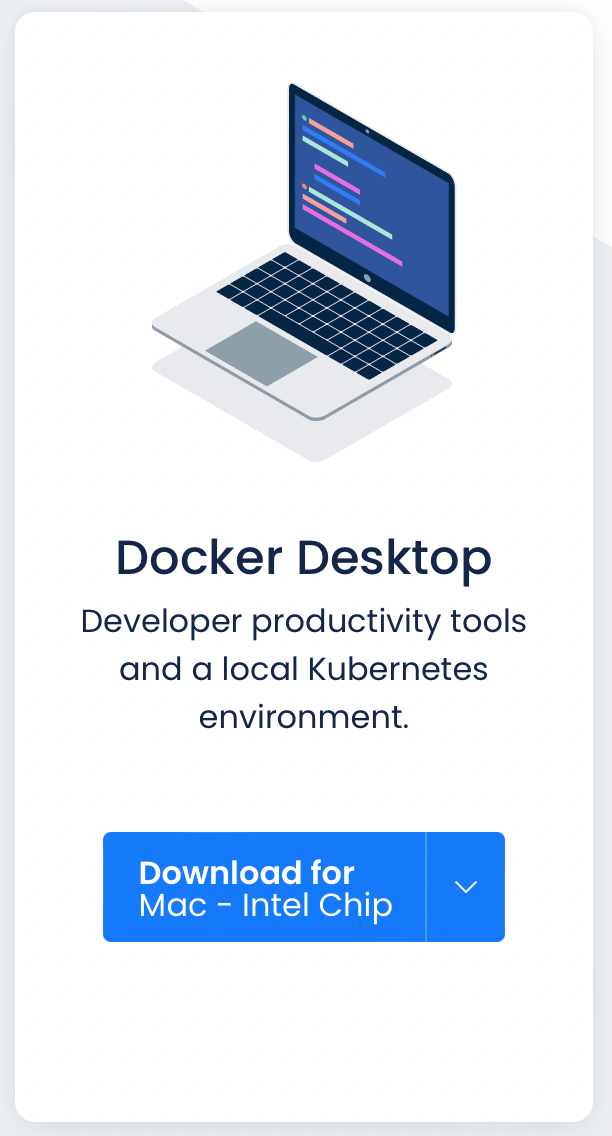
\includegraphics[height=90mm]{media/Handbuch/dockerdesktop.png}
    \caption{Installation von Docker}
\end{figure}

\hfour{Quellcode}

Entwickelt wurde \ZELIA\ mit Hilfe von Git und gelagert von GitHub. GitHub ist vereinfacht gesagt eine Plattform, auf der man Quellcode hosten kann, um gemeinsam daran mit Versions Kontrolle (Git) arbeiten zu können. 

Von GitHub kann man sich einfach mit Git oder "GitHub Desktop" den Quellcode lokal als Arbeitskopie auf einen Computer kopieren. Wenn man kein Git verwenden kann oder will kann man den gesamten Code auch als ZIP-File herunterladen. Durch die Verwendung von Git sieht man allerdings auf einem Blick ob und was sich an dem Quellcode bei Updates verändert hat.

\begin{figure}[H]
    \centering
    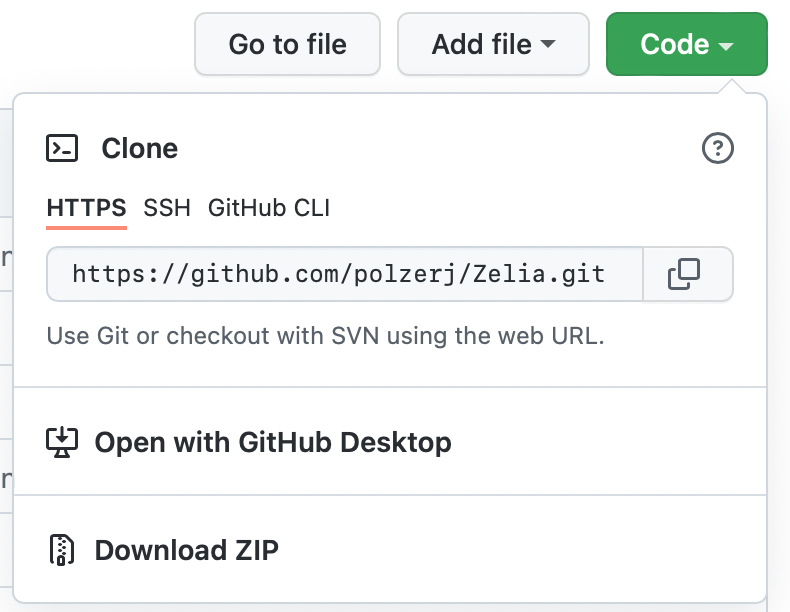
\includegraphics[width=100mm]{media/Handbuch/GitHub_Download.png}
    \caption{Herunterladen des Quellcodes von GitHub}
\end{figure}

\hfive{Git in der Kommandozeile}

In der Kommandoeingabe des jeweiligen Betriebssystem kann man sich mit dem einfachen Befehl \emph{git clone https://github.com/polzerj/Zelia.git} eine Arbeitskopie herunterladen. Dabei wird in dem Verzeichnis in dem man sich befindet ein Unterorder mit dem Namen "ZELIA" angelegt, in dem der gesamte Code liegt.

\hfive{GitHub Desktop}

Nachdem man das Programm geöffnet hat wird man gefragt von wo man eine Arbeitskopie holen will. Hier muss man auswählen \emph{Aus dem Internet kopieren} und dann die URL von dem Repository angeben (siehe Abbildung \ref{fig:clonewithdesktop}). Wenn man auf "Kopieren" gedrückt hat, wird der Quellcode in das ausgewählte Verzeichnis geladen. 

\begin{figure}[H]
    \centering
    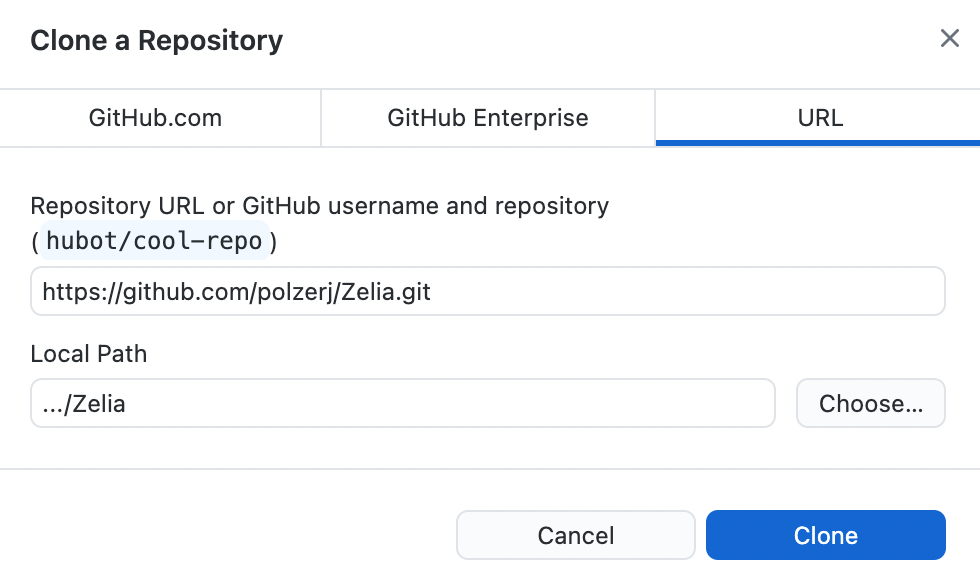
\includegraphics[width=100mm]{media/Handbuch/clone_gh.png}
    \caption{Quellcode mit "GitHub Desktop" herunterladen}
    \label{fig:clonewithdesktop}
\end{figure}

\hthree{Starten des Servers}

Wenn der Quellcode nun auf dem beliebigen Server herunterladen wurde, muss man noch eine \emph{.env-Datei} im Unterverzeichnis "api" anlegen, in der die notwendigen Umgebungsvariablen stehen. Diese werden benötigt um zu definieren auf welchem Port der Server läuft, welche Anmeldedaten für die Abfrage von WebUntis verwendet werden und noch vieles mehr (siehe Code \ref{fig:envexample}).


\begin{singlespace}
    \begin{lstlisting}[caption={Beispiel einer .env-Datei},label={fig:envexample},captionpos=b]
PORT=3001
DB_SERVER=db
DB_USER=***
DB_PASSWORD=***
DB_DATABASE=Zelia
WEBUNTIS_SCHOOL=szu
WEBUNTIS_USERNAME=***
WEBUNTIS_PASSWORD=***
WEBUNTIS_BASE_URL=aoide.webuntis.com
EMAIL_NAME=***
EMAIL_PASSWORD=***
JWT_SECRET=ZEL1A
    \end{lstlisting}
\end{singlespace}

\hfour{Entwicklung}

Wenn der Server im Entwicklungsmodus gestartet wird, kann bei einer Änderung im Quellcode der veränderte Programmteil automatisch neugestartet werden. Um den Server in diesem Zustand zu starten, muss man in dem ZELIA-Verzeichnis in den beiden Unterordern "pwa" und "api" jeweils folgendes Kommando in der Konsole ausführen: \emph{npm install} oder verkürzt \emph{npm i}. Dadurch werden vom "Node Packet Manager" (siehe Kapitel "NPM" \ref{sec:npm}) alle Bibliotheken heruntergeladen die benötigt werden um den Server zum Laufen zu bringen.

Danach muss man unter MacOS und Windows "Docker Desktop" öffnen, damit die "Docker-Engine" gestartet wird. Auf Linuxsystemen ist dieser Vorgang nicht notwendig (siehe Kapitel \ref{sec:dockerexplained}). Nachdem die "Docker-Engine" geladen wurde, kann man die Docker-Container mit folgendem Befehl starten:

\emph{docker-compose -f docker-compose.dev.yaml --env-file api/.env up}  

Beim ersten Mal wird der Startvorgang etwas länger dauern, da im Hintergrund die Abbilder der Docker-Container heruntergeladen werden.

\hfour{Produktion}

So wie im Entwicklungsmodus muss man auch hier "Docker Desktop" öffnen, um Docker verwenden zu können. Statt \emph{npm i} in den beiden Unterverzeichnissen ausführen zu müssen, startet man nur die Docker-Container mit folgendem Befehl:

\emph{docker-compose -f docker-compose.yaml --env-file api/.env up}

Auch dieser Startvorgang wird beim ersten Mal etwas länger dauern, da erstens Docker die notwendigen Abbildungen herunterlädt und zweitens der NPM-Installationsvorgang in den Docker-Containern ausgeführt wird.

Um zu überprüfen ob der Server erfolgreich gestartet wurde, kann man in einem Browser der Wahl probieren die API zu erreichen. 

\emph{https://localhost/api} oder im Entwicklungsmodus \emph{https://localhost:3001/api}.